%第2章:準備
%システムを開発する際,使用した定義.


本章では,研究方針のフローと,本論文で使用する用語について述べる.

\subsection*{V字開発モデル}

V字開発モデルとはソフトウェアの開発の流れを示したもののひとつである.
以下の図\ref{vji}にV字開発モデルの開発プロセスを示す.
横軸は開発の時間軸であり,縦軸は詳細化の程度を表している\cite{kumikomi}.
はじめに全体的な設計を行い,そこから詳細化した設計へと移る.
一方でテストに関しては部分部分のテストから全体のテストへと移っていく.
図\ref{vji}にも示すように,V字開発モデルにおいては,設計とテストが詳細化の程度の点で対応して行うものとなっている.
%詳細設計は単体テスト,基本設計は結合テストによって,要求分析は総合テストによって検証する.
各段階の設計に合わせたテストを計画,実施し,それが満たされているかを検証する.
%また,設計の段階で判明した不具合は,左側の対応する設計にさかのぼった作業を必要とする.
本研究では開発プロセスモデルとしてこのV字開発モデルを採用した.

\begin{figure}[htbp]
\centering
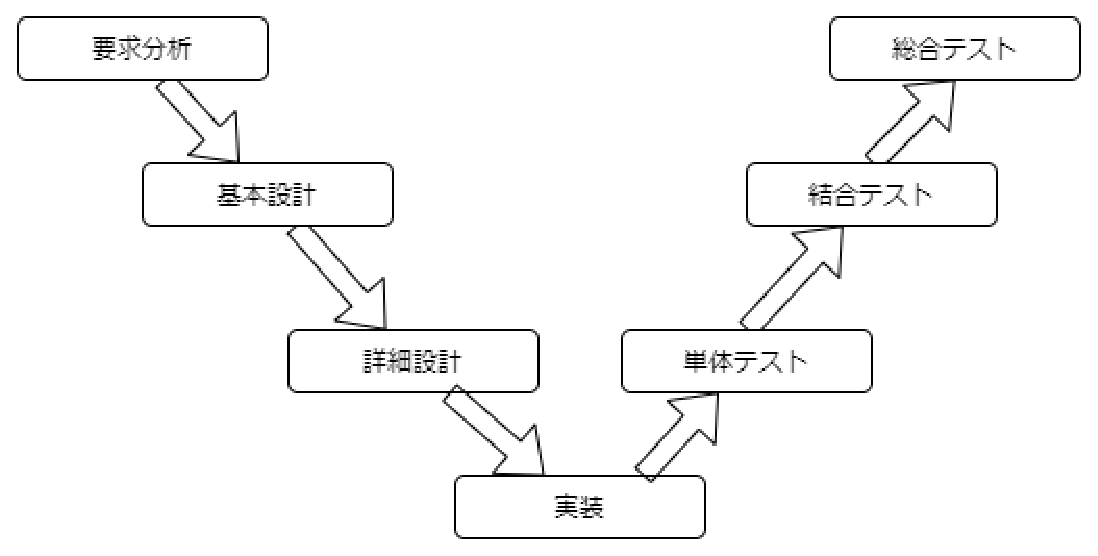
\includegraphics[width=10cm]{./picture/vjimodel.eps}
\caption{V字開発モデル}
\label{vji}
\end{figure}


\subsection*{UML(Unifiled Modeling Language)}

UMLとは統一モデリング言語(Unified Modeling Language)のことで,設計の仕様を表すものである\cite{uml}.
UMLにおいては設計の表現として,着目する点ごとに複数の図表が定義されている.
設計の内容を文字だけではなく図表によって表現しているため,顧客,および開発者間での統一した解釈を図れるようになっている.
UMLはOMG(Object Management Group)によって標準規格に認定されており,オブジェクト指向を用いたものとなっている\cite{uml}.
そのため,オブジェクトごとのカプセル化がなされ,再利用もしやすいという特長を持つ.

\subsection*{ユースケース図}

ユースケース図とは,UMLで定義されている図のうちのひとつである.
どのような機能を持っているのかということを外部からの視点で整理するために用いられる\cite{iot}.
システムがどのように機能すべきかという振る舞い(ユースケース)と,その外部環境(アクター)を表す\cite{uml}.
ユーザーから見てシステムがどのように動作しているのかを示したものがユースケース図である.

\subsection*{アクティビティ図}

アクティビティ図とは,UMLで定義されている図のひとつである.
ひとつの業務のワークフローを示したもの\cite{uml}であり,その処理がどのような順番で行われるのかが時系列に沿って示される.
処理の順番や並列処置の内容を示したものがアクティビティ図である.

\subsection*{クラス図}

クラス図はUMLの基本となる図のひとつである.
システム内のオブジェクトのうち共通部分のあるものをクラスとしてまとめ,それらの関係を示す.
システムや対象領域の静的な構造を表した図である.

\subsection*{シーケンス図}

シーケンス図とは,UMLで定義されている相互作用図のひとつである.
システム内でそれぞれのオブジェクトがどのようなやり取りを行うことで処理が進むのかを示したものであり,それを時間軸に沿って整理した図である.
オブジェクト間のメッセージのやり取りを時間の観点で表した図である.

\subsection*{ステートチャート図}

ステートチャート図とは,UMLで定義されている図のひとつである.
ひとつのオブジェクトの内部状態がイベントによってどのように変化していくのかを示した図法\cite{uml}であり,システム構成要素の状態遷移を示す.

\subsection*{IEEE802.15.4}

IEEE802.15.4とはIEEE(Institute of Electrical and Electronics Engineers)によって定義されている無線規格の一つである.
OSI参照モデルの物理層,およびデータリンク層の標準を定めている規格である.
近距離通信として無線PAN(Personal Area Newwork)に用いるものとして規定されている\cite{wnet}.
速度は250kbps,40kbps,20kbps\cite{ieee}と比較的遅いが,無認可で利用可能な周波数を用いているという特徴がある.
使用周波数については複数種類指定されているが,本研究においては日本での一般使用を想定しているため,920MHzおよび2.4GHzとして利用する.
電力管理により,低消費電力が実現できるという点が特長である.